\chapter{Prozess Architekturplanung}
Aufbauend auf den im Anforderungsprozess ermittelten Attribute, kann nun mit der Architekturplanung begonnen werden.

\section{Erstellen der Minimalen Architektur}
Das Kontext Diagramm, welches im Anforderungsprozess erstellt worden ist, zeigt das System mit allen Akteuren und Nachbarsystemen. Aufbauend darauf kann nun die minimale Architektur erstellt werden, welche sich aus dem System und den Nachbarsystemen ableitet.

\begin{figure}[H]
    \centering
    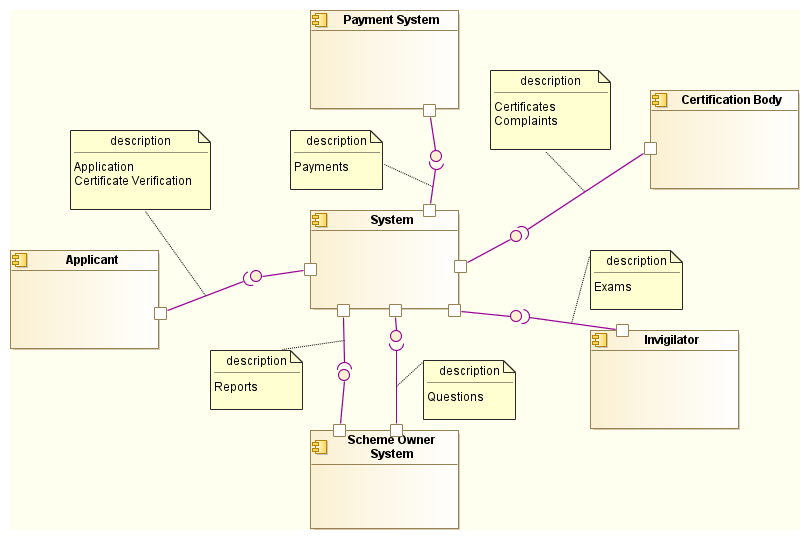
\includegraphics[scale=0.5]{uml/context.png}
    \caption{Das Kontext Diagramm liefert die Ausgangsbasis für die Architektur}
\end{figure}

Zuerst werden alle Datenflussnotizen entfernt. Danach werden alle Komponenten entfernt, welche kein eigenes System darstellen. In diesem Falle werden folgende Komponenten entfernt:

\begin{itemize}
  \item Applicant
  \item Certification Body
  \item Invigilator
\end{itemize}

Dies führt zu folgender Minimalarchitektur:

\begin{figure}[H]
    \centering
    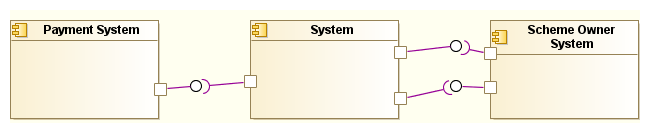
\includegraphics[scale=0.7]{uml/minimalarch.png}
    \caption{Minimale Architektur}
\end{figure}

Für die Nachbarsysteme wird keine Architektur erstellt, jedoch beinflussen sie die Schnittstellen des Systemes und sind deswegen wichtig für den weiteren Prozes. Sie werden in die Architektur einbezogen und in die niedrigste Vertrautheitsebene eingeteilt.

\section{Erstellen der Datenminimalarchitektur}
Auf Basis der Vertrautheitskategorien der Daten wird das System der vorher erstellte Minimalarchitektur in ebenso viele Teilsysteme unterteilt. Die Aktivitätsdiagramme werden an die neue Architektur angepasst: Für jedes Untersystem wird in den Diagrammen eine eigene Swimlane erstellt.

\begin{figure}[H]
    \centering
    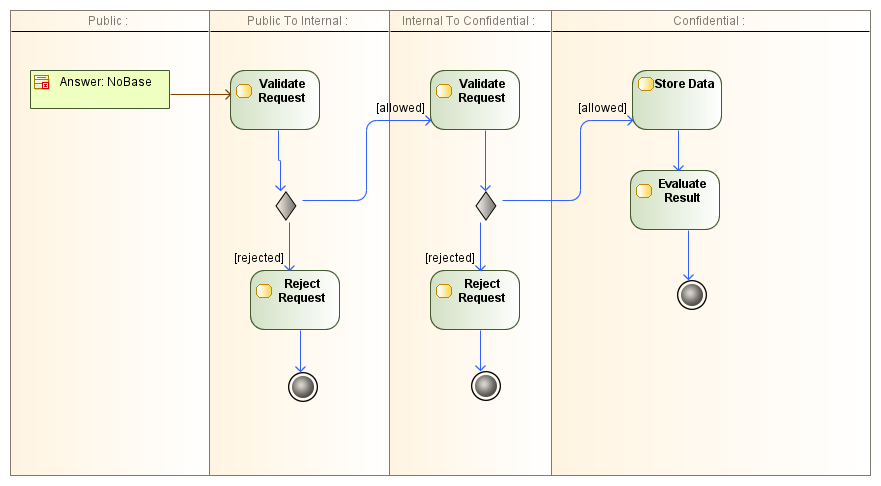
\includegraphics[scale=0.5]{uml/takeexamactivity1.png}
    \caption{Die Antworten werden nach der Prüfung an den Certification Body übermittelt. Der Request wird durch zwei Gateways zum finalen System geleitet.}
\end{figure}

Wechselt der Kontrollfluss eine Swimlane, heißt dies, dass eine Verbindung zwischen den beiden sonst abgeschotteten Systemen benötitgt wird. Dieses Verbindung wird als eigenes System modelliert und wird als Gateway bezeichnet. Die Aufgabe dieses Gateways ist es, folgende Attribute der Anfrage zu überprüfen und die Anfrage gegebenenfalls zu verwerfen oder weiterzuleiten:

\begin{itemize}
  \item Von welchem System kommt die Anfrage?
  \item Welches System ist das Ziel der Anfrage?
  \item Welche Schnittstelle dieses Systems ist das Ziel der Anfrage?
  \item Gibt es eine Regel die diese Anfrage explizit erlaubt?
\end{itemize}

\begin{figure}[H]
    \centering
    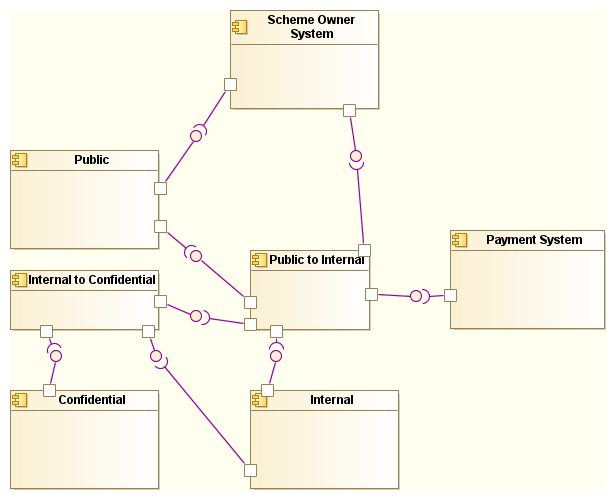
\includegraphics[scale=0.7]{uml/dataarch.png}
    \caption{Aufteilung der Komponenten in Datenbereiche}
\end{figure}

Wichtig ist hier, dass keine Gateways unterschiedlicher Vertrautheitsebenen übersprungen werden. Zeigt ein Aktivitäts Diagramm zB. einen Zugriff von Ebene 1 auf Ebene 3 muss dieser Zugriff sowohl durch den Gateway der Ebene 2 geleitet werden, als auch durch den Gateway der Ebene 3. Dies verhindert, dass besonders schützenswerte Systeme direkt an Systeme mit einem weitaus niedrigeren Vertrautheitsgrad angeschlossen werden und so dessen Gateway zum Single Point of Failure wird. Dies gilt in beide Richtungen.

Da bei der Erstellung des Systems alle Schnittstellen und Systeme bekannt sind, können diese Regeln fest im Gateway verankert werden. Weil diese Gateways unabhängig voneinander agieren, können sie durch das Hinzufügen eines Load Balancers beliebig vervielfacht werden, was sowohl die Ausfallsicherheit als auch die Skalierbarkeit erhöht. Das ist wichtig, weil sie als einzige Verbindung zwischen den Systemen zu einer Art Flaschenhals werden.


\section{Einbinden der Akteure}
Nachdem die Datenminimalarchitektur steht, können nun die Akteure des Systems mit einbezogen werden. Hierfür müssen nun die Objektflüsse des Systems betrachtet werden, welche aus dem Aktivitätsdiagramm ersichtlich sind.

TODO: modelio objektflüsse zeigen

Zuerst wird das erste Untersystem, in diesem Falle das Public System, betrachtet. Alle dort eingehenden Anfragen und deren Objekte werden im Moment durch dieses einzelne System verwaltet und gegebenenfalls weiter geleitet, was durch die unterschiedlichen Akteure und deren Vertrautheit in den meisten Fällen ein Sicherheitsproblem darstellt. Deswegen wird das Untersystem in den allermeisten Fällen in weitere Teilsysteme aufgespaltet werden müssen.

Die Grundidee hinter dieser Aufspaltung ist folgende: Je mehr Aufgaben das System übernehmen muss, desto mehr potentielle Angriffsfläche bietet es Angreifern (TODO: zitat). Jeder Akteur der auf das System zugreifen kann, kann das System auch angreifen. Deswegen muss das System so gestaltet sein, dass bei einer kompletten Kontrolle des Systems durch einen Akteur der Schaden so gering wie möglich ausfällt.

Idealerweise würde deswegen die Anzahl der einzelnen Systeme gleich der Anzahl der Akteure in diesem System sein. Dies hätte jedoch zur Folge, dass auch für triviale Angriffe komplette Systeme entstehen würden, deren Erstellung und Wartung mehr kosten könnten als der tatsächlich daraus resultierende Schaden.

TODO: algorithmus zur aufspaltung erstellen

TODO: modelio teile des systems, beispielaufteilung zeigen

Ist ein Untersystem fertig aufgespalten, wird nun mit dem nächsten Untersystem fortgefahren, bis alle behandelt wurden.

\section{Modellieren der Komponenten Interfaces (Klassen Diagramm)}
Aufzeigen dass zb das interne System user anlegen können muss mit methoden im klassendiagramm

\section{Analyse der nicht funktionalen Attribute}
Auf Basis von dokumentierten Szenarien können nun nicht funktionale Attribute gemessen werden und Hinweise kritische/wichtige Komponenten gegeben werden. Kostengegenüberstellung können auch eigene Systeme rechtfertigen/entfernen

\subsection{Reliability}
Single Point of Failure Analyse (Matrix Komponente x Usecase), Erklären wie man auf Matrix kommt (Aktivitätsdiagramm), Ausfallskosten (inkl. Wachstumsszenarien)

Einfache Methode zur schätzung der Ausfallkosten, aufzeigen wie durch Reduzieren der Ausfallswahrscheinlichkeit Kosten sinken aber auch Investitionskosten verursachen. Wachstumsszenarien auch einbeziehen in die Rechnung
\subsection{Usability}
In diesem Teil des Prozesses nicht wichtig, da noch keine Implementierung vorhanden.

\subsection{Efficiency}
Efficiency kann pro usecase gemessen werden, zb für antwortzeiten indem man zb die swimlanewechsel der Aktivitätsdiagramme zählt und mit einer konstanten multipliziert (geschätzte Netzwerkgeschwindigkeit). Ansonsten ist es durch die fehlende Implementation nicht möglich die Geschwindigkeit oder den Arbeitsspeicherverbrauch zu messen.

\subsection{Maintainability}
Auslesbar aus der Usecase Matrix, als Summe aller subsysteme,

\subsection{Portability}
In diesem Teil des Prozesses nicht wichtig, da noch keine Implementierung vorhanden.
